\documentclass[12pt]{article}

\usepackage[top=3cm,bottom=3cm]{geometry}
\geometry{a4paper}

\usepackage{polyglossia}
\setdefaultlanguage{french}
\usepackage{csquotes}
\usepackage{unicode-math}
%\usepackage{fontspec}
\usepackage{xltxtra}
\usepackage{amsmath}
%\setmathfont{texgyretermes-math.otf}
\setmainfont[Ligatures=Rare]{Linux Libertine O}%

\renewcommand{\textsc}{}

\usepackage[htt]{hyphenat}
\usepackage{subcaption}

\usepackage{amsopn}
\usepackage{stmaryrd} %% llbracket
\usepackage{algorithm2e}

\usepackage{float}

\newenvironment{algorithme}[1][t]
  {\renewcommand{\algorithmcfname}{Algorithme}% Update algorithm name
   \begin{algorithm}[#1]%
  }{\end{algorithm}}


% Macros
\usepackage{xparse}
\usepackage{xifthen} % \ifthenelse

\newtheorem{theorem}{Théorème}[section]
\newtheorem{definit}{Définition}[section]
\newtheorem{corollary}{Corollaire}[theorem]
\newtheorem{lemma}[theorem]{Lemme}

\usepackage{tabularx}
\newcolumntype{Y}{>{\centering\arraybackslash}X}
\usepackage{multirow}


%%%% Imiter Mlapafr2 avec Bibtex %%%%
%% TODO: éliminer les attributs superflus pour la bibliographie
\usepackage[backend=biber,style=authoryear-comp,uniquename=init,firstinits=true,
            %% "et al" pour > deux auteurs, & pour exactement 2
            uniquelist=false,maxcitenames=2,mincitenames=1,maxbibnames=99,
            isbn=false,url=false,doi=false
]{biblatex}

\DeclareSourcemap{
  \maps[datatype=bibtex]{
    \map{
      \step[fieldsource=series,
        match={\regexp{\s}}, replace={\regexp{\\nobreakspace\x20}}]
      }
  }
}

\renewcommand{\cite}{\parencite}
\renewcommand*{\nameyeardelim}{\addcomma \addnbspace}
% \renewcommand*{\multinamedelim}{\space} % fait le contraire de ce qu'on veut
\renewcommand*{\revsdnamedelim}{}
\renewcommand*\finalnamedelim{ \& }

\DefineBibliographyExtras{french}{\restorecommand\mkbibnamelast}

\DeclareNameAlias{default}{last-first}
\DeclareNameAlias{sortname}{last-first}

% Supprimer les guillemets dans les titres
\DeclareFieldFormat[article,incollection,unpublished,inproceedings]{title}{#1}

% Je n'aime pas, mais j'ai l'impression que mlapafr utilise ça
\renewbibmacro{in:}{\printtext{In} \addspace}


% Espaces insécables dans les citations et la bibliographie (noms de
% conférences) ?

\usepackage{xpatch}
\usepackage{xstring}
%\xpatchbibmacro{series+number}{\addspace}{\addnbspace}{}{}

\renewbibmacro*{series+number}{%
  \setunit*{\addnbspace}%
  \printfield{series}%
  \printfield{number}%
  \newunit}


\xpatchbibmacro{textcite}{\addcoma}{}{}{}

\addbibresource{references.bib}

\usepackage{hyperref}
\usepackage{xspace} % Espaces après macros


\usepackage{todonotes}
\newcommand{\question}[1]{\todo[color=green!40]{#1}}
\newcommand{\questioni}[1]{\todo[color=green!40,inline]{#1}}


%%%% Macros Arthur %%%%
\newcommand{\diff}[2]{\frac{\partial{}{#1}}{\partial{}{#2}}}

\usepackage{mathtools}
\DeclarePairedDelimiterX\setc[2]{\{}{\}}{#1 \;\delimsize\vert\; #2}

\newcommand\mimic{\texttt{MIMIC-III} }
\newcommand\wordtovec{\texttt{Word2Vec} }
\newcommand\doctovec{\texttt{Doc2Vec} }
\newcommand\wordpieces{\emph{word pieces} }
\newcommand\bow{\emph{bag of words} }
\newcommand\skipgram{\emph{skip-gram} }
\newcommand\cbow{\emph{CBOW} }
\newcommand\batchnorm{\emph{batch normalization} }
\newcommand\bert{\emph{BERT} }

\newcommand{\contrainte}[1]{($\text{C}_{#1}$)}


% Notation suites mathématiques
%% 3 options - nécessite xparse !
%% \newcommand{\nsuite}[3][i][N]{({#3}_{#1})_{#1=1}^{#2}}
\DeclareDocumentCommand{\nsuite}{ O{N} O{i} m }
  {({#3}_{#2})_{#2=1}^{#1}}

% Notation pour 'la matrice X sans la colonne j'
\newcommand{\matremov}[2]{%
  %%Substitution i et j !
  \StrSubstitute{#2}{j}{\jmath}[\temp]%
  \StrSubstitute{\temp}{i}{\imath}[\tempp]%
  #1_{\hat{\tempp}
  }
}

% Cardinal
\newcommand{\card}[1]{\left\vert{#1}\right\vert}

% Intervalles
\NewDocumentCommand{\INTERVALINNARDS}{ m m }{
    #1 {,} #2
}
\NewDocumentCommand{\inter}{ s m >{\SplitArgument{1}{,}}m m o }{
    \IfBooleanTF{#1}{
        \left#2 \INTERVALINNARDS #3 \right#4
    }{
        \IfValueTF{#5}{
            #5{#2} \INTERVALINNARDS #3 #5{#4}
        }{
            #2 \INTERVALINNARDS #3 #4
        }
    }
}

%% intervalle entier
\newcommand{\ninter}[2]{\llbracket #1...#2 \rrbracket}

% Transposée

\makeatletter
\newcommand*{\transpose}{%
  {\mathpalette\@transpose{}}%
}
\newcommand*{\@transpose}[2]{%
  % #1: math style
  % #2: unused
  \raisebox{0.2em}{$\m@th#1\intercal$}%
}
\makeatother

%% FIXME : pas tout à fait la bonne notation
%% Voir ISO 80000-2 §2-15.7
%% \newcommand*{\tran}{^{\mkern-1.5mu\mathsf{T}}} ?
\newcommand{\tr}[1]{ {#1}^{\! \transpose}}

% Gras
% Précaution pour les lettres avec exposant : voir mathspec !
% FIXME : le " fait buguer \emph ???
\newcommand{\mb}[1]{{\boldsymbol{\mathbf{#1}}}}

% Distance à base de norme

\newcommand*{\newvarcmd}[2]{%
  \newcommand*{#1}[2][]{%
    \begingroup % \sizel and \sizer are local:
      \let\varl\left
      \let\varr\right
      \ifthenelse{\isempty{##1}}{%
        \let\sizel\relax
        \let\sizer\relax
      }{%
        \expandafter\let\expandafter\sizel\csname ##1l\endcsname
        \expandafter\let\expandafter\sizer\csname ##1r\endcsname
      }%
      #2%
    \endgroup
  }
}

\newvarcmd{\abs}{\sizel\lvert #2\sizer\rvert}
\newvarcmd{\norm}{\sizel\lVert #2\sizer\rVert}
\newcommand{\dist}[2]{\norm{#1 - #2}}

%% Macro pour les vecteurs directeurs
\NewDocumentCommand{\vdir}{ m O{j} O{r} }{\mb{#1}_{#3#2}}
\newvarcmd{\primabs}{\sizel\lvert #2\sizer\rvert}

\renewcommand{\eqref}[1]{équation~\ref{#1}}
\newcommand{\algref}[1]{algorithme~\ref{#1}}
\newcommand{\figref}[1]{figure~\ref{#1}}
\newcommand{\tabref}[1]{tableau~\ref{#1}}
\newcommand{\secref}[1]{section~\ref{#1}}

\AtBeginDocument{ %Bizarrerie unicode-math
  \DeclareMathOperator{\mmin}{\mathrm{min}}
  \DeclareMathOperator{\mmax}{\mathrm{max}}
  \DeclareMathOperator{\eexp}{\mathrm{exp}}
  \DeclareMathOperator{\argmin}{\text{argmin}}
  \newcommand{\gargmin}[2]{\argmin_{#1}\left\{{#2}\right\} }
  \DeclareMathOperator{\prox}{\mathrm{prox}}
  \newcommand{\proxg}[3]{\prox_{\frac{#1}{#2}{#3}}}
}

\begin{document}
\title{REDS - TP2 : Baseline et méthode d'ensemble}
\author{Laura Nguyen et Keyvan Beroukhim}
\maketitle

Toujours à partir des données issues du \emph{ATLAS Higgs Boson Machine Learning
Challenge 2014}, l'objectif durant ce TP est d'établir une baseline pour la
prédiction du type d'évènement : \emph{s} pour \emph{signal} et \emph{b} pour
\emph{background}.

Avant de mettre en place des modèles d'apprentissage, les données doivent être
nettoyées. On supprime d'abord les attributs \texttt{KaggleSet},
\texttt{Weight}, \texttt{KaggleWeight} et \texttt{EventId}. Ensuite, les
features contenant plus de 40\% de valeurs manquantes sont supprimées. Enfin, on
retire les évènements à valeurs manquantes. On passe d'un dataset de 818238 à
693636 échantillons (environ 85\% des données initiales) et de 35 à 20
attributs.

Par souci de temps de calcul, les expériences suivantes sont menées sur le
dataset restreint à 10000 évènements. 70\% de cette base est dédiée à
l'entraînement et la validation des modèles, 30\% au test. 

On évaluera les performances des modèles avec l'accuracy, le score F1 et le
score AMS.

\section{Baseline}

On établit dans un premier temps une baseline : les évènements seront classifiés
à l'aide d'un SVM linéaire. Pour trouver la valeur optimale de l'hyperparamètre
$C$, on effectue un \emph{grid search} sur l'ensemble $\{10^{-4}, 10^{-3},
10^{-2}, 10^{-1}, 1, 10, 100, 1000\}$. Pour chaque valeur, un SVM est entraîné
par \emph{cross-validation} sur 4 folds. Moyenner les scores obtenus sur chaque
fold permet d'avoir une bonne estimation de la performance du modèle en
apprentissage. Pour chacune des trois mesures d'évaluation, la
\figref{fig:svm-scores} contient la courbe des performances moyennes produites
avec chaque $C$.

\begin{figure}[H]
	\centering
    \begin{subfigure}[c]{0.45\textwidth}
        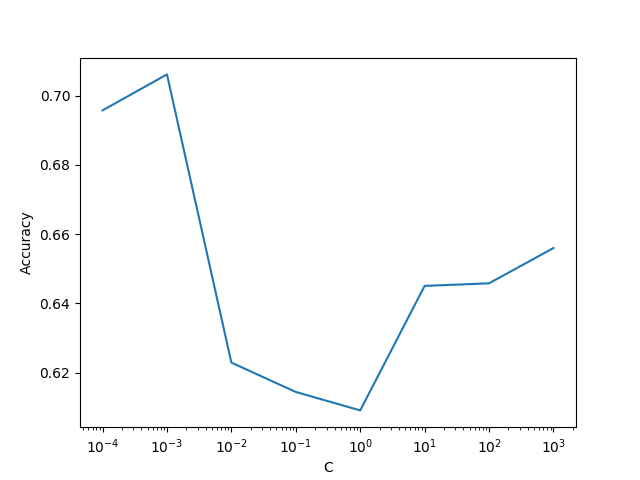
\includegraphics[width=\textwidth]{images/accuracy.png}
    \caption{Accuracy}
    \end{subfigure}
    \begin{subfigure}[c]{0.45\textwidth}
        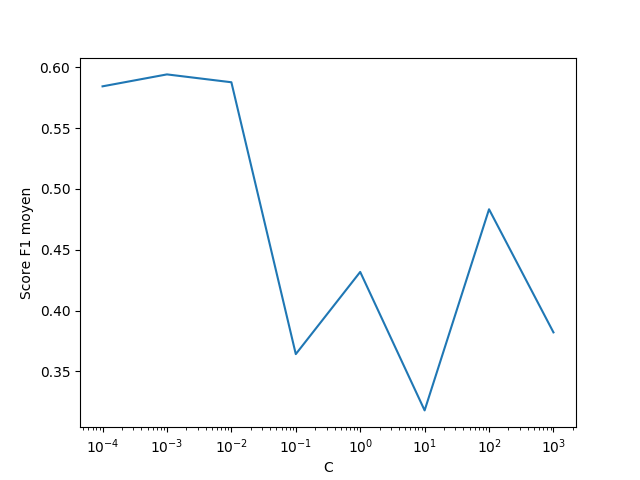
\includegraphics[width=\textwidth]{images/f1.png}
    \caption{Score F1}
    \end{subfigure}

    \begin{subfigure}[c]{0.45\textwidth}
        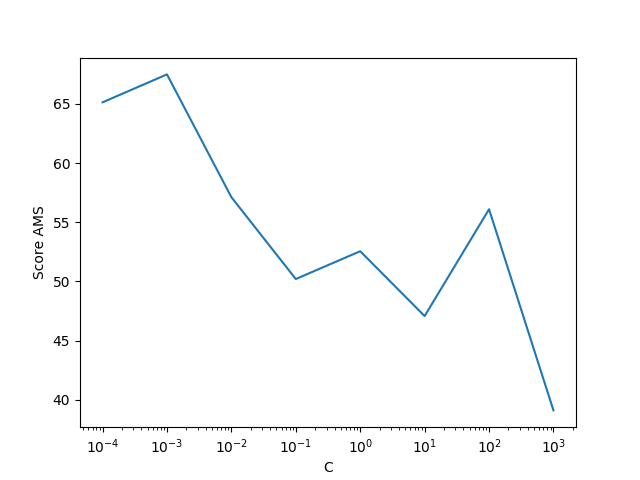
\includegraphics[width=\textwidth]{images/ams.png}
    \caption{AMS}
    \end{subfigure}

    \caption{Performances moyennes en apprentissage en fonction de $C$}
    \label{fig:svm-scores}
\end{figure}

On récupère la valeur de $C$ permettant d'obtenir le meilleur score F1 moyen sur
les données d'entraînement. Un SVM est ensuite entraîné avec cette valeur sur
l'ensemble d'entraînement. Pour chaque mesure d'évaluation, les performances en
apprentissage et en test figurent dans le \tabref{tab:results-SVM}.

\begin{table}[H]
\centering
\resizebox{0.6\textwidth}{!}{
\begin{tabular}{c|c|c|c|c}
         & Accuracy & Score F1 & AMS \\
        \hline
        Apprentissage & 70.82\% & 58.47\% & 134.95\\
        Test & 70.69\% & 58.20\% & 87.74\\
\end{tabular}}
\caption{Scores obtenus en apprentissage et en test}
\label{tab:results-SVM}
\end{table}

\section{Méthodes d'ensemble}

On utilise maintenant plusieurs méthodes d'ensemble dans l'objectif d'améliorer
les performances :

\begin{itemize}
    \item \emph{Bagging} avec un \emph{Perceptron} comme classifieur faible
    \item \emph{Random Forest}
    \item \emph{AdaBoost}
\end{itemize}

Comme chacune de ces méthodes possède un nombre important d'hyperparamètres et
qu'un grid search serait donc coûteux, on définit arbitrairement leurs valeurs.

Chaque classifieur est entraîné sur la totalité des données d'entraînement puis
évalué sur l'ensemble de test. Les résultats en apprentissage et en test
figurent dans le \tabref{tab:ensemble-results}.


\begin{table}[H]
    \resizebox{1.15\textwidth}{!}{
        \begin{tabular}{c|*{5}{c|}c}
            \multirow{2}{*}{} &
            \multicolumn{2}{c|}{Accuracy} &
            \multicolumn{2}{c|}{F1} &
            \multicolumn{2}{c}{AMS}\\ \cline{2-3} \cline{4-5} \cline{6-7}
            & Apprentissage & Test  & Apprentissage & Test & Apprentissage & Test \\
            \hline
            Random Forest & 94.91\% & 80.00\% & \% & \% &  & \\
        \end{tabular}}
    \caption{Performances obtenues par chaque méthode}
    \label{tab:ensemble-results}
\end{table}

%\begin{table}[H]
%\resizebox{1.15\textwidth}{!}{
%    \begin{tabular}{c|*{5}{c|}c}
%        \multirow{2}{*}{} &
%        \multicolumn{2}{c|}{Accuracy} &
%        \multicolumn{2}{c|}{F1} &
%        \multicolumn{2}{c}{AMS}\\ \cline{2-3} \cline{4-5} \cline{6-7}
%        & Apprentissage & Test  & Apprentissage & Test & Apprentissage & Test \\
%        \hline
%        Bagging & 68.74\% & 67.17\% & 40.49\% & 38.44\% & 35.04 & 23.12 \\
%        Random Forest & 98.66\% & 78.07\% & 97.97\% & 69.10\% & 140.71 & 35.10 \\
%        AdaBoost & 80.43\% & 78.00\% & 74.19\% & 72.03\% & 58.06 & 35.06 \\
%\end{tabular}}
%\caption{Performances obtenues par chaque méthode}
%\label{tab:ensemble-results}
%\end{table}

\end{document}
